\documentclass{beamer}
\usepackage{beamerthemeshadow}
\usepackage[ruled]{algorithm}
\usepackage{listings}
%\usepackage[font=scriptsize]{subcaption}
\usepackage[font=scriptsize]{caption}
\usepackage[noend]{algpseudocode}

\settowidth{\leftmargini}{\usebeamertemplate{itemize item}}
\addtolength{\leftmargini}{\labelsep}

\renewcommand{\thefootnote}{\fnsymbol{footnote}}
\setbeamerfont{footnote}{size=\tiny}

\captionsetup[figure]{labelformat=empty}

\graphicspath{ {./figure/} }


\begin{document}
\title[Logarithmic Search Data Structure Based on MDList]{An Efficient Lock-free Logarithmic Search Data Structure Based on Multi-dimensional List}
\author[D. Zhang \and D. Dechev]{Deli Zhang \and Damian Dechev}
\institute{Department of Computer Science\\ 
University of Central Florida}

\date{\today}

\begin{frame}
    \titlepage
\end{frame}

\begin{frame}
    \frametitle{Table of Contents}
    \tableofcontents
\end{frame}

\section{Introduction}
\subsection{Overview}
\begin{frame} \frametitle{Concurrent Dictionary}
    \begin{itemize}
        \item Abstract Data Type
            \begin{itemize}
                \item Supports \textsc{Insert}, \textsc{Delete}, and \textsc{Find}
                \item Keys are totally ordered
            \end{itemize}
        \item Typical Implementations
            \begin{itemize}
                \item Binary Search Trees (BST)
                \item Skip-lists
                \item Hash Tries
            \end{itemize}
        \item Lock-freedom
            \begin{itemize}
                \item Scalable fine-grained synchronization
                \item Fault tolerance 
            \end{itemize}
    \end{itemize}
\end{frame}

\subsection{Search Data Structures}
\begin{frame} \frametitle{Lock-free BST}
    \begin{itemize}
        \item Node not found $\neq$ Key not found
            \begin{itemize}
                \item Embed logical ordering [Drachsler et al. 2014]
                \item Use external (leaf-oriented) trees [Ellen et al. 2010]
            \end{itemize}
        \item Balancing induces bottleneck
            \begin{itemize}
                \item Relaxed balancing [Bronson et al. 2010]
                \item Background balancing [Crain et al. 2013]
            \end{itemize}
    \end{itemize}
    \begin{figure}[H]
        \centering
        \includegraphics<1>[width=6cm]{bst-find.pdf}
        \footnote{Illustration from Drachsler et al. 2014}
    \end{figure}
\end{frame}

\begin{frame} \frametitle{Lock-free Skip-list}
    \begin{itemize}
        \item Probabilistically balanced alternative
            \begin{itemize}
                \item Bottom level linked list
                \item Redundant short-cut links
                \item Exponentially lower probability
            \end{itemize}
        \item Concurrency limitation [Fraser 2004, Crain et al. 2013]
            \begin{itemize}
                \item \textsc{Insert}/\textsc{Delete} update multiple nodes
            \end{itemize}
    \end{itemize}
    \begin{figure}[H]
        \centering
        \includegraphics<1>[width=1\textwidth]{Skip_list_svg.png}
        \footnote{Illustration from wikipedia}
    \end{figure}
\end{frame}

\begin{frame} \frametitle{Lock-free Tries}
    \begin{columns}
        \begin{column}{7cm}
            \begin{itemize}
                \item Ctrie [Prokopec et al. 2012] 
                    \begin{itemize}
                        \item A hash array mapped trie
                        \item Value stored internally
                        \item Hot spot: Intermediate (I) nodes
                    \end{itemize}
                \item SkipTrie [Oshman and Shavit 2013]
                    \begin{itemize}
                        \item Y-fast trie with skip-list
                        \item Require double-word CAS
                        \item Value stored externally
                        \item Hot spot: inserting prefixes
                    \end{itemize}
            \end{itemize}
        \end{column}
        \begin{column}{5cm}
            \begin{figure}[H]
                \centering
                \includegraphics<1>[width=1\textwidth]{./ctrie-insert.pdf}
                \caption{Ctrie Insert}
            \end{figure}
            \vspace{-1.2cm}
            \begin{figure}[H]
                \centering
                \scalebox{1.0}[1.2]{\includegraphics<1>[width=1\textwidth]{./skiptrie.pdf}}
                \caption{SkipTrie\footnotemark}
            \end{figure}
        \end{column}
    \end{columns}
    \footnotetext{Illustration from Prokopec et al. 2012, and Oshman and Shavit 2013}
\end{frame}

\subsection{Motivation}
\begin{frame} \frametitle{}
    \begin{itemize}
        \item What makes an efficient lock-free dictionary?
            \begin{itemize}
                \item Low branching factor --- avoids hot spots
                \item Localized updates --- reduces access conflicts
                \item Fixed key positions --- simplifies predecessor query
            \end{itemize}
        \item Proposed Multi-dimensional List (MDList)
            \begin{itemize}
                \item Lower level nodes have smaller branching factor
                \item \textsc{Insert}/\textsc{Delete} modifies at most 2 adjacent nodes
                \item Unique layout per logical ordering  
                \item No balancing/randomization required 
                \item Memory efficient
            \end{itemize}
    \end{itemize}
\end{frame}

\section{Algorithm}
\subsection{Intuition}
\begin{frame} \frametitle{Ordered Linked List}
\begin{columns}
        \begin{column}{6.5cm}
            \begin{figure}[H]
                \centering
                \includegraphics<1>[width=1\textwidth]{./mdlist-1d.pdf}
            \end{figure}
        \end{column}
        \begin{column}{5.5cm}
            \begin{itemize}
                \item Re-arranged into columns
                \item Partitioned sub-lists
                \item $\mathcal{O}(N)$ \textsc{Find}
            \end{itemize}
        \end{column}
    \end{columns}
\end{frame}

\begin{frame} \frametitle{Ordered 2D List}
\begin{columns}
        \begin{column}{6.5cm}
            \begin{figure}[H]
                \centering
                \includegraphics<1>[width=1\textwidth]{./mdlist-2d.pdf}
            \end{figure}
        \end{column}
        \begin{column}{5.5cm}
            \begin{itemize}
                \item Short-cut links on top 
                \item Vector coordinates $(d_0, d_1)$ 
                \item Lexicographical ordering
                \item Worst-case $\mathcal{O}(\sqrt N)$ \textsc{Find}
            \end{itemize}
        \end{column}
    \end{columns}
\end{frame}

\subsection{Definition}
\begin{frame} \frametitle{Multi-dimensional List}
    \begin{definition}
    A $D$-dimensional list is a tree in which each node is implicitly assigned a dimension of $d \in [0,D)$. The root node's dimension is $0$. A node of dimension $d$ has no more than $D-d$ children, where the $m$th child is assigned a dimension of $d'=d+m-1$.
    \end{definition}
    \begin{definition}
    Given a non-root node of dimension $d$ with coordinate $\mathbf{k}=(k_0,...,k_{D-1})$ and its parent with coordinate $\mathbf{k'}=(k'_0,...,k'_{D-1})$ in an ordered $D$-dimensional list: $k_i = k'_i, \;\forall \;i \in [0, d) \land k_d > k'_d$.
    \end{definition}
\end{frame}

\begin{frame} \frametitle{Coordinate Mapping}
\begin{columns}
        \begin{column}{7cm}
            \begin{figure}[H]
                \centering
                \includegraphics<1>[width=1\textwidth]{mdlist-3d.pdf}
            \end{figure}
        \end{column}
        \begin{column}{5.3cm}
            \begin{itemize}
                \item $k \mapsto (d_0, d_1, ..., d_{D-1})$ 
                \item \emph{Injective} and \emph{monotonic}
                \item Preferably uniform
                \item Base conversion: choose $base=\lceil\sqrt[D]{U}\;\rceil$
                    \begin{example}
                        $U=64,D=3,base=4$\\
                        $(63)_{10}=(333)_{4}$\\
                        $(34)_{10}=(202)_4$
                    \end{example}
            \end{itemize}           
        \end{column}
    \end{columns}
\end{frame}

\subsection{Operations}
\begin{frame} \frametitle{Find Operation}
\begin{columns}
        \begin{column}{7cm}
            \begin{figure}[H]
                \centering
                \includegraphics<1>[width=1\textwidth]{mdlist-3d.pdf}
            \end{figure}
        \end{column}
        \begin{column}{5.3cm}
             \begin{itemize}
                 \item Recursively traverse sub-lists  
                 \item Comparing coordinates from $d=0$ 
                 \item Worst-case $\mathcal{O}(D \sqrt[D]{n})$ time
                 \item Choose $D = \log{U}$ then $\mathcal{O}(\log{U} \sqrt[\log{U}]{U}) = \mathcal{O}(\log{U})$
             \end{itemize}           
        \end{column}
    \end{columns}
\end{frame}

%\begin{frame} \frametitle{Locate Unique Inserting Position}
%\begin{columns}
        %\begin{column}{7cm}
            %\begin{figure}[H]
                %\centering
                %\includegraphics<1>[width=1\textwidth]{mdlist-3d-ins-1.pdf}
            %\end{figure}
        %\end{column}
        %\begin{column}{5cm}
            %\begin{itemize}
                %\item Compare coordinate vector from $d=0$
                %\item Increase $d$ if equal
                %\item Go to $d$th child if greater 
                %\item Stop if smaller
            %\end{itemize}
        %\end{column}
    %\end{columns}
%\end{frame}

\begin{frame} \frametitle{Insert --- 2 Steps}
    \begin{columns}
        \begin{column}{7cm}
            \begin{figure}[H]
                \centering
                \includegraphics<1>[width=1\textwidth]{mdlist-3d-ins-1.pdf}
                \includegraphics<2>[width=1\textwidth]{mdlist-3d-ins-2.pdf}
            \end{figure}
        \end{column}
        \begin{column}{5.3cm}
            \begin{enumerate} 
                \item Pointer swing
                    \begin{itemize}
                        \item Predecessor query locate $pred,curr,d_p,d_c$
                        \item CAS updates $pred.child[d_p]$
                    \end{itemize}
                \item<2> Child adoption
                    \begin{itemize}
                        \item Necessary if $d_c \neq d_p$ 
                        \item $curr.child[d_p:d_c]$ transferred to new node
                        \item Use descriptor for helping in case process is delayed
                    \end{itemize}
            \end{enumerate} 
        \end{column}
    \end{columns}
\end{frame}

\begin{frame} \frametitle{Normal Delete --- 2 steps}
    \begin{columns}
        \begin{column}{7cm}
            \begin{figure}[H]
                \centering
                \includegraphics<1>[width=1\textwidth]{mdlist-3d-del-1.pdf}
                \includegraphics<2>[width=1\textwidth]{mdlist-3d-del-2.pdf}
            \end{figure}
        \end{column}
        \begin{column}{5.3cm}
            \begin{enumerate} 
                \item Prompt the next node 
                    \begin{itemize}
                        \item Examine coordinates from $D-1$ 
                        \item Swing $pred$'s pointer
                    \end{itemize}
                \item<2> Child transfer
                    \begin{itemize}
                        \item Inverse of child adoption  
                        \item Potential conflicts
                    \end{itemize}
            \end{enumerate} 
        \end{column}
    \end{columns}
\end{frame}

\begin{frame} \frametitle{Normal Delete Does Not Work}
    \begin{itemize}
        \item \textsc{Insert} may demote a node (i.e., increase its dimension)
        \item \textsc{Delete} may promote a node (i.e., decrease its dimension)
\begin{alertblock}{Synchronization Issue}
        Due to the helping mechanism, several threads may execute child adoption on the same node.
        Without additional synchronization, we cannot know if all of them have finished.
        Data races may arise among ongoing child adoption and child transfer processes.
    \end{alertblock}
        \item Solution: Keep dimension change \emph{unidirectional} 
    \end{itemize}
\end{frame}

\begin{frame} \frametitle{Asymmetrical Delete --- Decoupled Physical Removal}
    \begin{columns}
        \begin{column}{7cm}
            \begin{figure}[H]
                \centering
                \includegraphics<1>[width=1\textwidth]{mdlist-3d-asmdel-1.pdf}
                \includegraphics<2>[width=1\textwidth]{mdlist-3d-asmdel-2.pdf}
            \end{figure}
        \end{column}
        \begin{column}{5.3cm}
            \begin{enumerate} 
                \item Mark for logical deletion 
                    \begin{itemize}
                        \item Still valid for routing 
                    \end{itemize}
                \item<2> \textsc{Insert} purge marked node 
                    \begin{itemize}
                        \item Adopt children in $[d_p,D)$  
                    \end{itemize}
            \end{enumerate} 
            \begin{itemize}
                \item<2> Reuse child adoption
                \item<2> Unifies help protocol
                \item<2> Simplifies synchronization
            \end{itemize}
        \end{column}
    \end{columns}
\end{frame}

\subsection{Correctness}
\begin{frame} \frametitle{Abstract State}
    \begin{figure}[h]
        \centering
        \includegraphics<1>[width=0.8\textwidth]{mdlist-abstract_state.pdf}
    \end{figure}
    \begin{itemize}
        \item The abstract state of the dictionary $S = M \setminus P$ 
        \item Linearization points
            \begin{itemize}
                \item \textsc{Insert}: when CAS updates predecessor's child pointer
                \item \textsc{Delete}: when CAS marks predecessor's child pointer
                \item \textsc{Find}: when predecessor's child pointer is read
            \end{itemize}
    \end{itemize}
\end{frame}

\section{Experiments}
\subsection{Setup}
\begin{frame} \frametitle{Environment}
    \begin{itemize}
        \item Hardware
            \begin{itemize}
                \item 64-core NUMA (4 AMD Opteron @2.1GHz)
                \item 6-core (12 w/ Hyper-threading) SMP (Intel Xeon @2.9GHz)
            \end{itemize}
        \item Software
            \begin{itemize}
                \item GCC 4.7 w/ O3
                \item Disabled memory reclamation
                \item Uses thread-caching malloc
            \end{itemize}
        \item Micro-benchmark
            \begin{itemize}
                \item Write-dominated, read-dominated, and mixed workloads
                \item 1K, 1M, and 1G key universes
            \end{itemize}
    \end{itemize}
\end{frame}

\begin{frame} \frametitle{Alternatives}
    \begin{itemize}
        \item BST
            \begin{itemize}
                \item Lock-based relaxed AVL by Bronson et al. (BRNBST)
                \item Lock-free unbalanced BST by Ellen et al. (ELNBST)
                \item RCU-based Citrus tree by Arbel et al. (CTRBST)
            \end{itemize}
        \item Skip-list (max tower height 30)
            \begin{itemize}
                \item Lock-free skip-list by Fraser (FRLIST)
                \item Lock-free skip-list by Herlihy (HLLIST)
                \item Lock-free rotating skip-list by Dick et al. (RTLIST)
            \end{itemize}
        \item MDList (dimension 16)
    \end{itemize}
    \footnotetext{BRNBST, ELNBST, and HLLIST are based on \\C++ implementation by Wicht et al. 2012}
\end{frame}

\subsection{Performance}
\begin{frame} \frametitle{Throughput --- NUMA Write-dominated Workload}
    \begin{columns}
        \begin{column}{8cm}
            \begin{figure}[t]
                \centering
                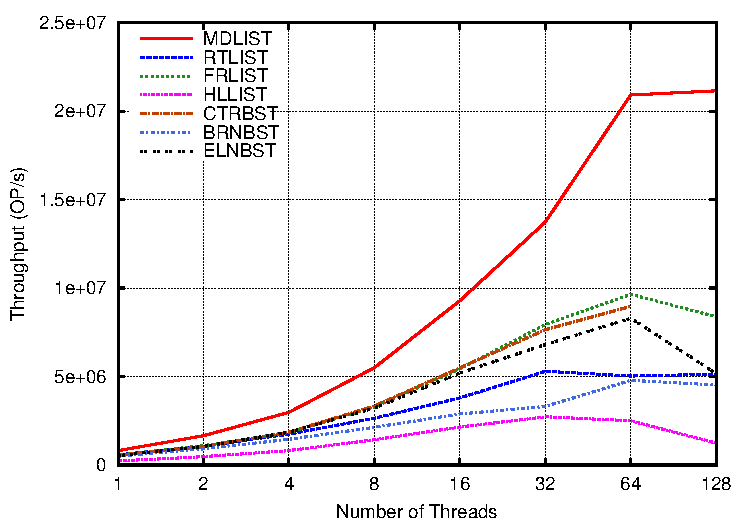
\includegraphics[width=1\columnwidth]{amd50ins1Bkey.pdf}
                \caption{1G Keys, 50\% \textsc{Insert} 50\% \textsc{Delete}}
                \end{figure}
            \end{column}
            \begin{column}{4.3cm}
                \begin{itemize}
                    \item As much as 100\% speedup for 64 threads
                    \item Optimized by localized node modifications
                \end{itemize}
            \end{column}
        \end{columns}
\end{frame}

\begin{frame} \frametitle{Throughput --- NUMA Mixed Workload}
    \begin{columns}
        \begin{column}{8cm}
            \begin{figure}[t]
                \centering
                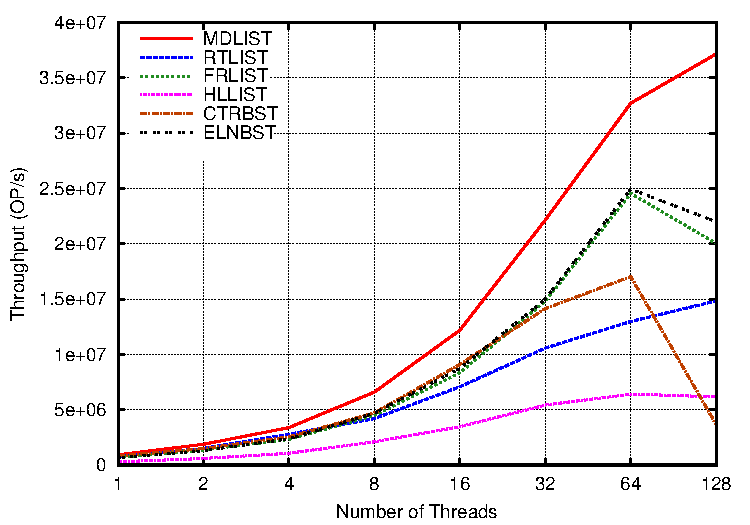
\includegraphics[width=1\columnwidth]{amd20ins1Mkey.pdf}
                \caption{1M Keys, 20\% \textsc{Insert} 10\% \textsc{Delete} 70\% \textsc{Find}}
                \end{figure}
            \end{column}
            \begin{column}{4.3cm}
                \begin{itemize}
                    \item As much as 50\% speedup for 64 threads
                \end{itemize}
            \end{column}
        \end{columns}
\end{frame}

\begin{frame} \frametitle{Throughput --- NUMA Read-dominated Workload}
    \begin{columns}
        \begin{column}{8cm}
            \begin{figure}[t]
                \centering
                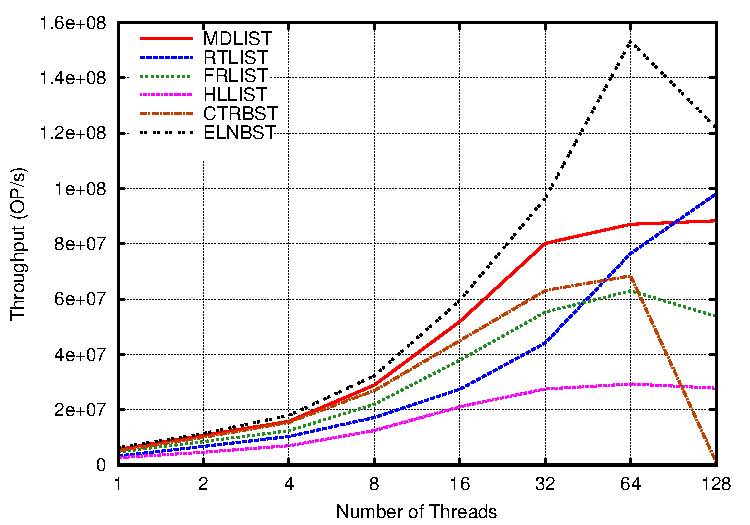
\includegraphics[width=1\columnwidth]{amd9ins1Kkey.pdf}
                \caption{1K Keys, 9\% \textsc{Insert} 1\% \textsc{Delete} 90\% \textsc{Find}}
                \end{figure}
            \end{column}
            \begin{column}{4.3cm}
                \begin{itemize}
                    \item BSTs have shallow depth
                    \item 16 dimension is too much for 1000 keys
                \end{itemize}
            \end{column}
        \end{columns}
\end{frame}

\begin{frame} \frametitle{Throughput --- SMP Mixed Workload}
    \begin{columns}
        \begin{column}{8cm}
            \begin{figure}[t]
                \centering
                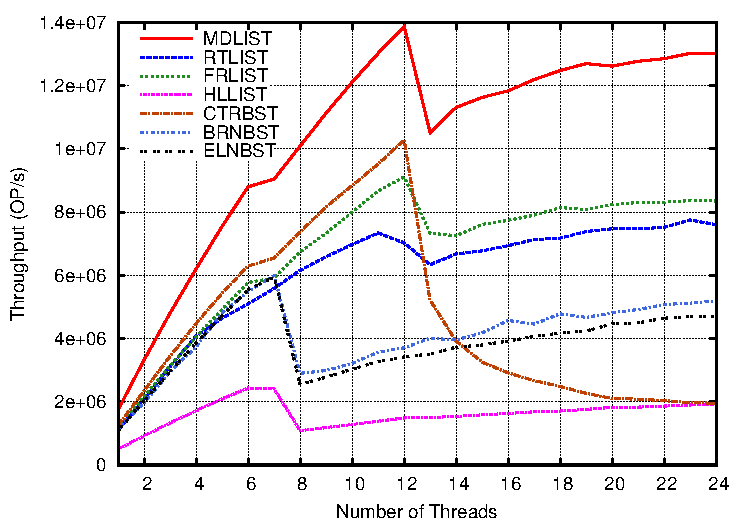
\includegraphics[width=1\columnwidth]{intel30ins4Mkey.pdf}
                \caption{1M Keys, 30\% \textsc{Insert} 20\% \textsc{Delete} 50\% \textsc{Find}}
                \end{figure}
            \end{column}
            \begin{column}{4.3cm}
                \begin{itemize}
                    \item 40\% speedup for 12 threads
                    \item Able to exploit hyper-threading
                \end{itemize}
            \end{column}
        \end{columns}
\end{frame}

\subsection{Tuning}
\begin{frame} \frametitle{Dimension Sweep}
    \begin{columns}
        \begin{column}{8cm}
            \begin{figure}[t]
                \centering
                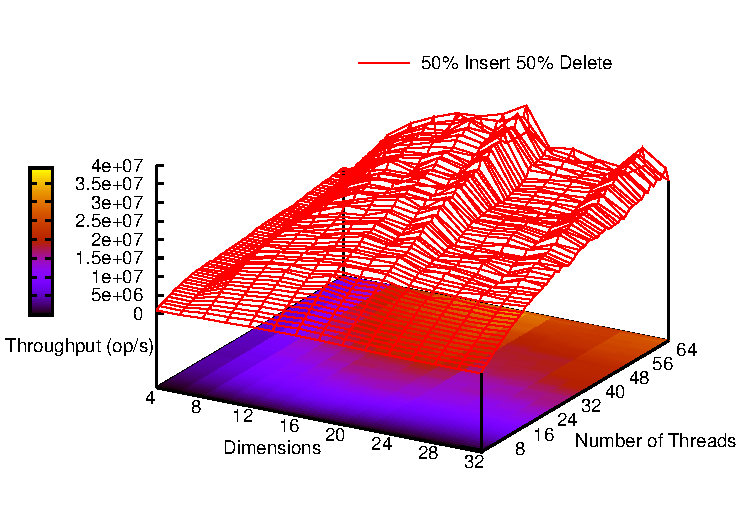
\includegraphics[width=1\columnwidth]{amdsweep50ins.pdf}
                \caption{1M Keys, 50\% \textsc{Insert} 50\% \textsc{Delete}}
                \end{figure}
            \end{column}
            \begin{column}{4.3cm}
                \begin{itemize}
                    \item For any number of threads, max throughput occurs when $D=20$
                    \item Performance of MDList is workload dependent and concurrency independent
                \end{itemize}
            \end{column}
        \end{columns}
\end{frame}


\section{Conclusion}
\begin{frame} \frametitle{Summary}
    \begin{itemize}
        \item Performance characteristics
            \begin{itemize}
                \item Excels at high level of concurrency and large key space
                \item Optimized for write operations
                \item Tuning based on workload and key space is possible
            \end{itemize}
        \item<2,3> Memory overhead per key-value pair
            \begin{itemize}
                \item Sequential: $D + 4$ bytes --- cached coordinates and child pointer
                \item Lock-free: additional $10$ bytes --- child adoption descriptor 
            \end{itemize}
        \item<3> Different key partition from tries
            \begin{center}
            \footnotesize
            \begin{tabular}{ | c | l | l | p{5cm} |}
            \hline
            Type & Minimal Key & Branching Factor & Common Prefix Length\\ \hline
            MDList & In root node & $K=D-d$ & $L = d' \in [d,D)$ \\ \hline
            Trie & In left-most leaf & $K$ is constant & $L = d$ for all children\\
            \hline
            \end{tabular}
            \end{center}
        \end{itemize}
\end{frame}

%\begin{center}
%\small
%\begin{tabular}{ | c | c | c | c | c | c |}
%\hline
%Type & Key Space & Order & Find & Insert & Space \\ \hline
%MDList & Fixed & Prefix & $\mathcal{O}(\log{U}) $ & $\mathcal{O}(\log{U}) $ & $\mathcal{O}(N)$ \\
%Skip-list & Fixed & key & $\mathcal{O}(\log{U}) $ & $\mathcal{O}(\log{U}) $ & $\mathcal{O}(2N)$ \\
%BST & Dynamic & key & $\mathcal{O}(\log{U}) $ & $\mathcal{O}(\log{N}) $ & $\mathcal{O}(N)$ \\
%SkipTrie & Fixed & Prefix & $\mathcal{O}(\log{\log{U}}) $ & $\mathcal{O}(\log{U}) $ & $\mathcal{O}(N)$ \\
%vEB Tree & Fixed & Prefix & $\mathcal{O}(\log{U}) $ & $\mathcal{O}(\log{U}) $ & $\mathcal{O}(N)$ \\
%\hline
%\end{tabular}
%\end{center}

\begin{frame}
    \begin{center}
        \large
Questions? \\
\bigskip
Thank you!
    \end{center}
\end{frame}

\end{document}
